\documentclass{article}
\usepackage{graphicx} % For including images
\usepackage{titling}  % For custom title page
\usepackage{circuitikz}
\usepackage{amsmath}
\usepackage{amssymb}
\usepackage{booktabs,tabu}
\usepackage[all, cmtip]{xy}
\newcommand{\ohm}{\Omega}
% Set up title and author
\title{Experiment 4: Frequency Modulation}
\author{Samyak Sheersh,Souhardya Bose,Aryam Shankar}
\date{27 August 2024}
\newcommand{\subtitle}[1]{%
  \posttitle{%
    \par\end{center}
    \begin{center}\large#1\end{center}
    \vskip0.5em}%
}

\begin{document}

% Custom title page
\begin{titlepage}
    \centering
    
\includegraphics[width=0.2\textwidth]{KGP_logo.png}\par\vspace{1cm}
    {\scshape\LARGE Department of Electronics and Electrical Communication Engineering, IIT Kharagpur\par}
    \vspace{1cm}
    {\huge\bfseries Experiment 4: Frequency Modulation\par}
    \vspace{1.5cm}
    {\Large\itshape Samyak Sheersh, Souhardya Bose, Aryam Shankar\par}
    \vfill
    % Identifying information at the bottom
    {\large Roll Numbers: 22EC30045, 21EE10097, 22EC3FP37\par}
    {\large Group Number: 12\par}
    \vfill
    {\large \today \par}
\end{titlepage}



\section{Objectives}
\emph{To realize frequency modulation using XR-2206. Observe both time domain
and frequency domain plots on DSOs for various scenarios.}
\begin{figure}[!ht]
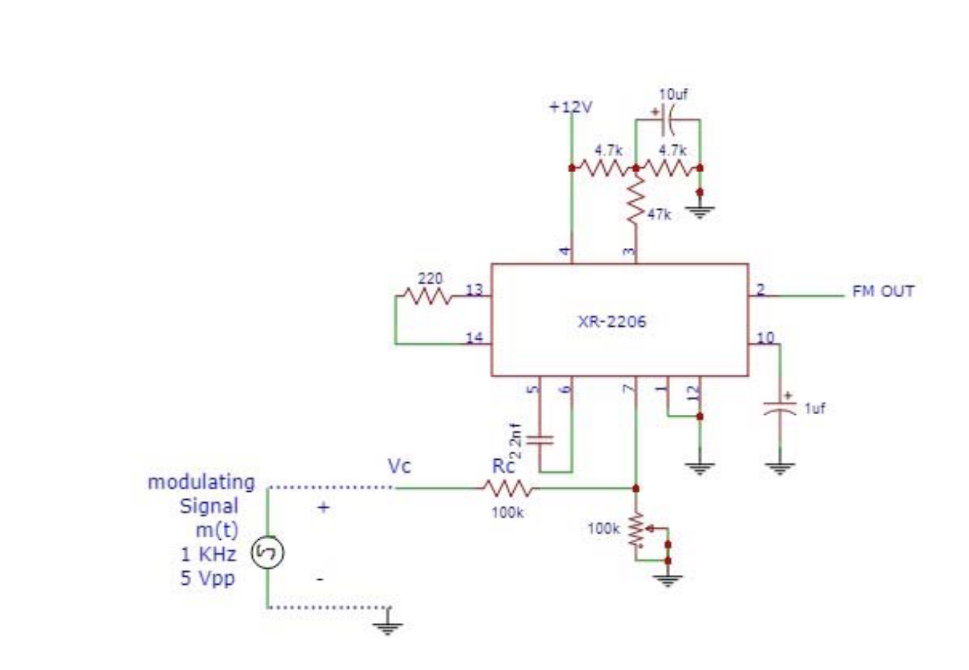
\includegraphics[width=\textwidth]{FM_using_ic.png}
\caption{Frequency modulation using XR-2206}
\label{fig:fm_circuit}
\end{figure}
\section{Instruments and Materials Used}
\begin{enumerate}
  \item RIGOL Signal Generator
  \item ScientiFIC SMO10C Digital Signal Oscilloscope
  \item +12V, -12V DC source and ground
  \item MC 1496 integrated circuit
  \item Resistors
  \item Capacitors
  \item Diodes
  \item Breadboard
  \item Connecting wires
\end{enumerate}
\section{Brief Theory and Procedure}
In frequency modulation, the final signal is of the form:
\begin{equation}
    V(t)=A\cos(2\pi f_i(t)t)
\end{equation}
where $f_i=f_c+k_fm(t)$

We define frequency deviation as: $\Delta f=f_{i,max}-f_c$

And the modulation index as:
\begin{equation}
  m=\frac{\Delta f}{f_m}    
\end{equation}
where $f_m$ is the highest frequency of the messaging signal.

We calculated the $f_{max}$ of the signal using two methods:
\begin{enumerate}
  \item By calculating the time difference between consecutive peaks in the densest region and then using:$f_{max}=\frac{1}{T_{min}}$
  \item By looking at the FFT and noting down the right-most peak.
\end{enumerate}

\section{Observations and Results}
\subsection{Carrier Wave}
\begin{figure}[!ht]
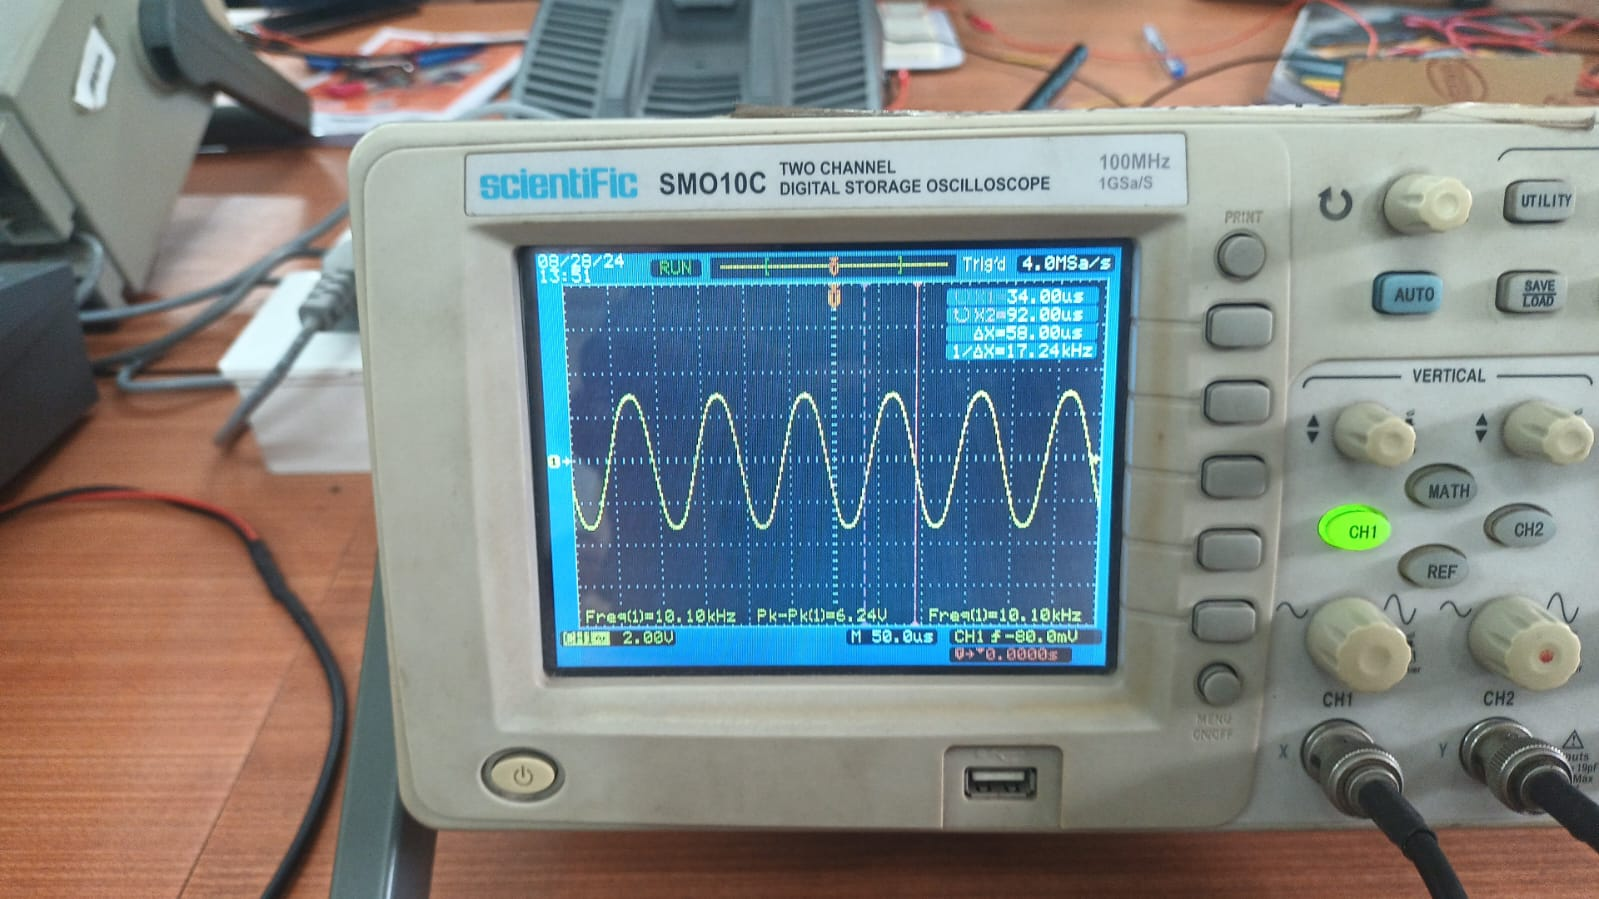
\includegraphics[width=\textwidth]{Carrier_10.08kHz.jpeg}
\caption{Carrier wave with frequency $f_c=10.08$ kHz and $V_{pp}=6.24V$}
\label{fig:carrier}
\end{figure}
\clearpage
\subsection{Modulated Signal}
\begin{figure}[!hbt]
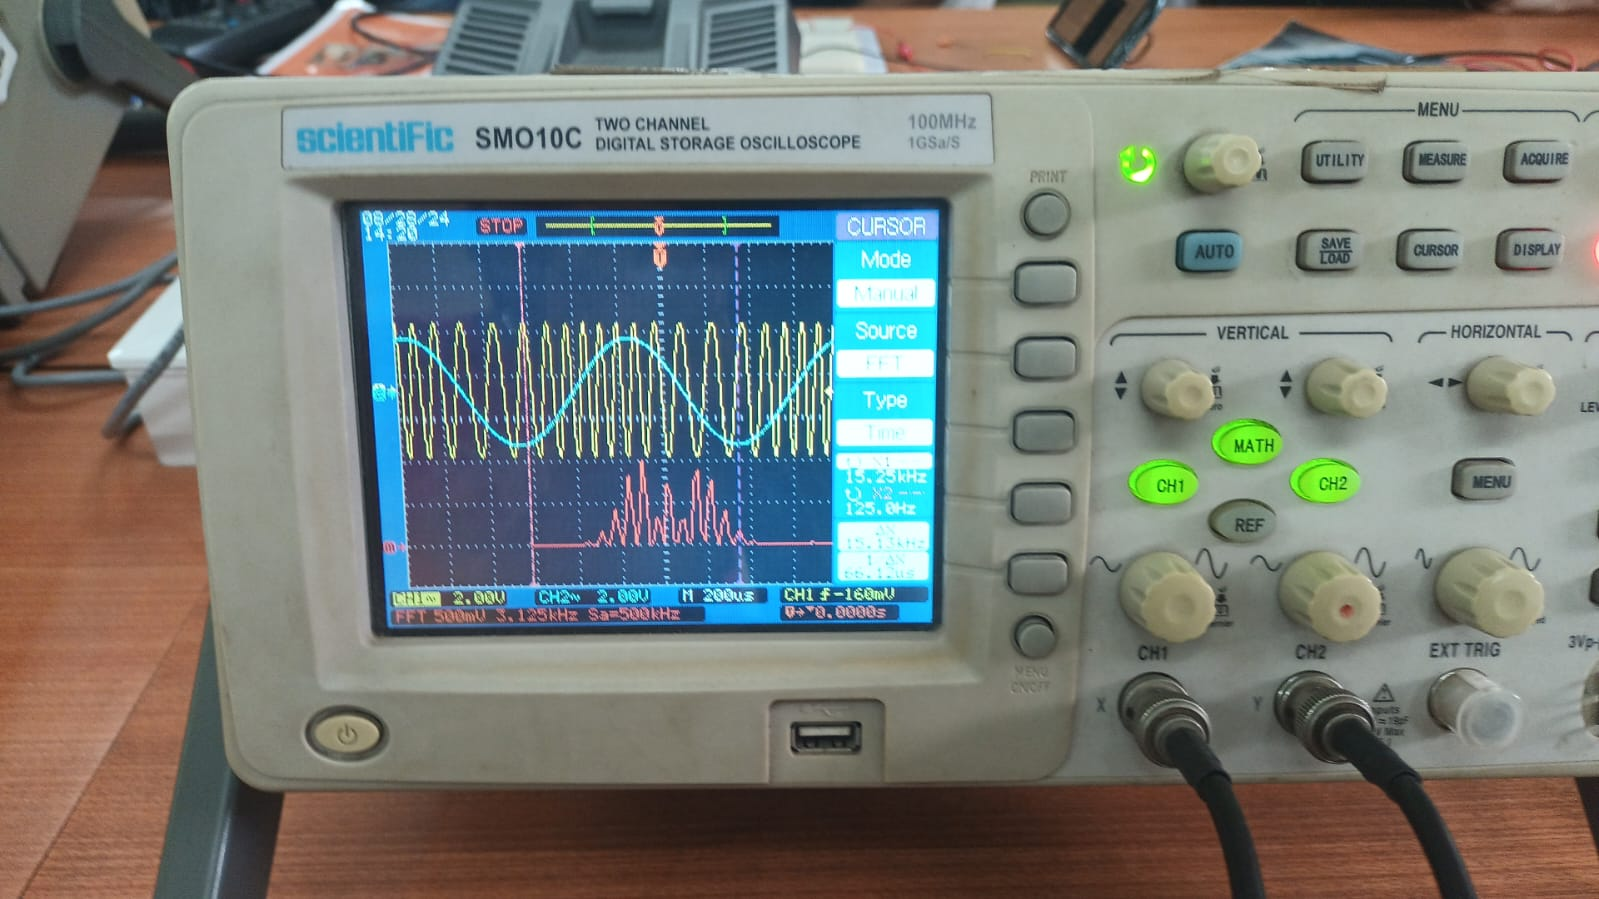
\includegraphics[width=\textwidth]{FM_mt_FFT.jpeg}
\caption{Frequency modulated output with $V_{pp}=5V, f_m=1kHz$, and corresponding FFT}
\label{fig:fm_mt_FFT}
\end{figure}
From the measurements in time domain:
$f_{max}=13.89kHz, f_{min}=8.621kHz$

From measurements in the frequency domain i.e. using the FFT:
$f_{max}=15.25kHz, f_{min}=5.25kHz$

Since the measurements from the FFT aregoing to be more accurate, we will use that to calculate the modulation index:
\begin{equation}
  m=\frac{\Delta f}{f_m}=\frac{f_{max}-f_c}{f_m}=\frac{15.25-10.08}{1}=5.17
\end{equation}
\clearpage
\subsection{Varying the amplitude}
\begin{figure}[!ht]
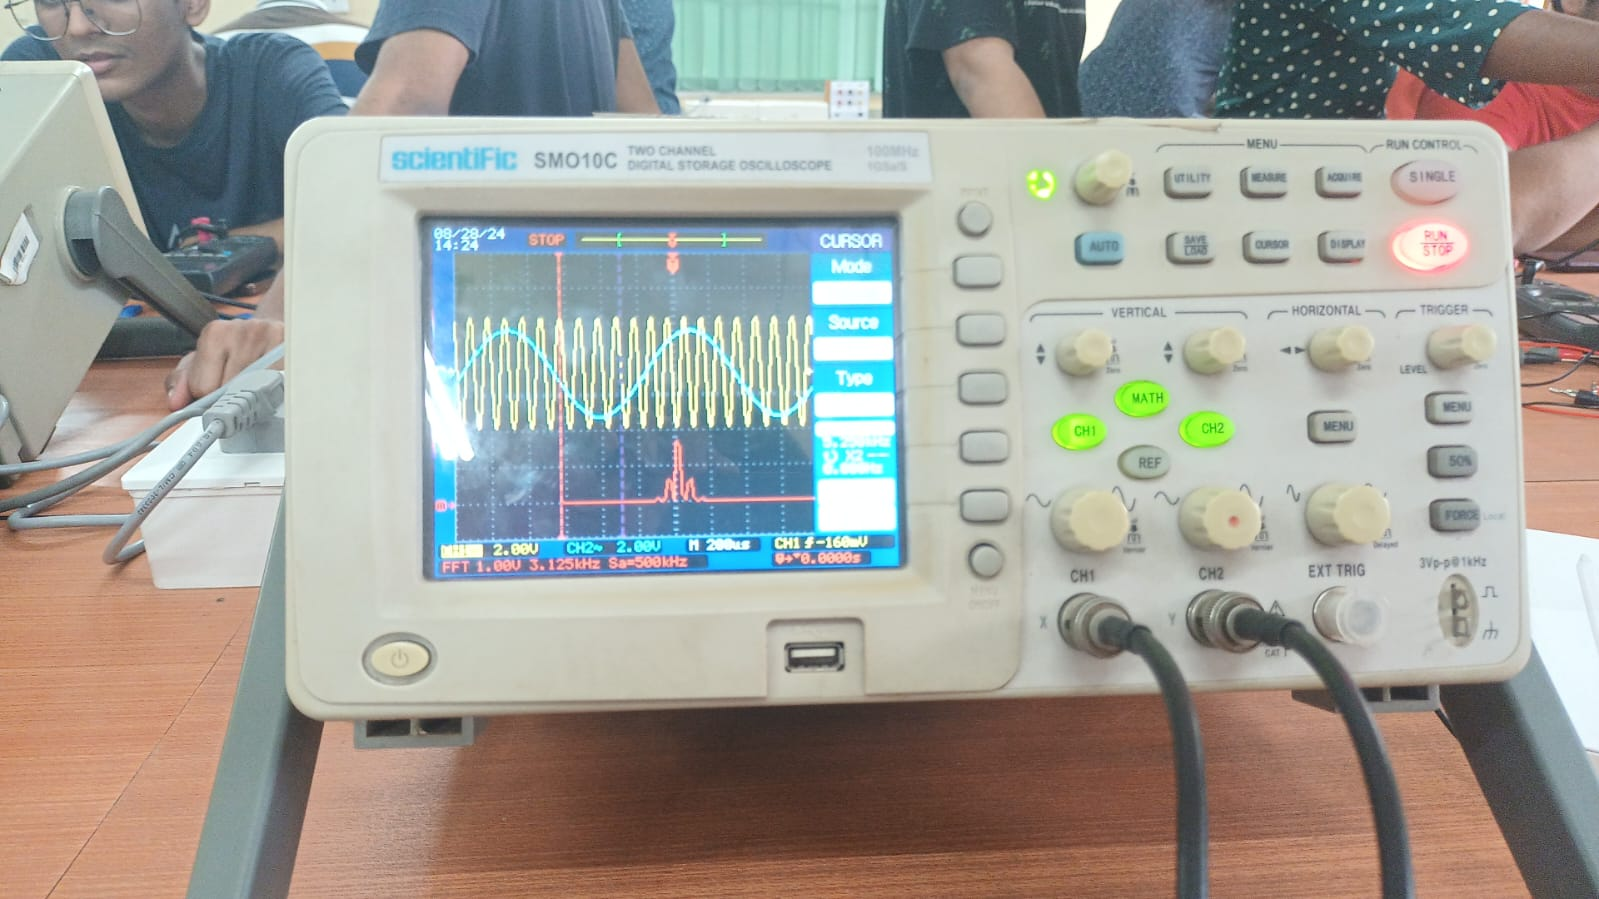
\includegraphics[width=\textwidth]{V_pp_m_1V.jpeg}
\caption{Final output and FFT with $V_{pp}=1V$ for the message}
\label{fig:V_pp_m_1V}
\end{figure}
\begin{equation}
    m=\frac{\Delta f}{f_m}=\frac{11.25-10.08}{1}=1.17
\end{equation}
\begin{figure}[!ht]
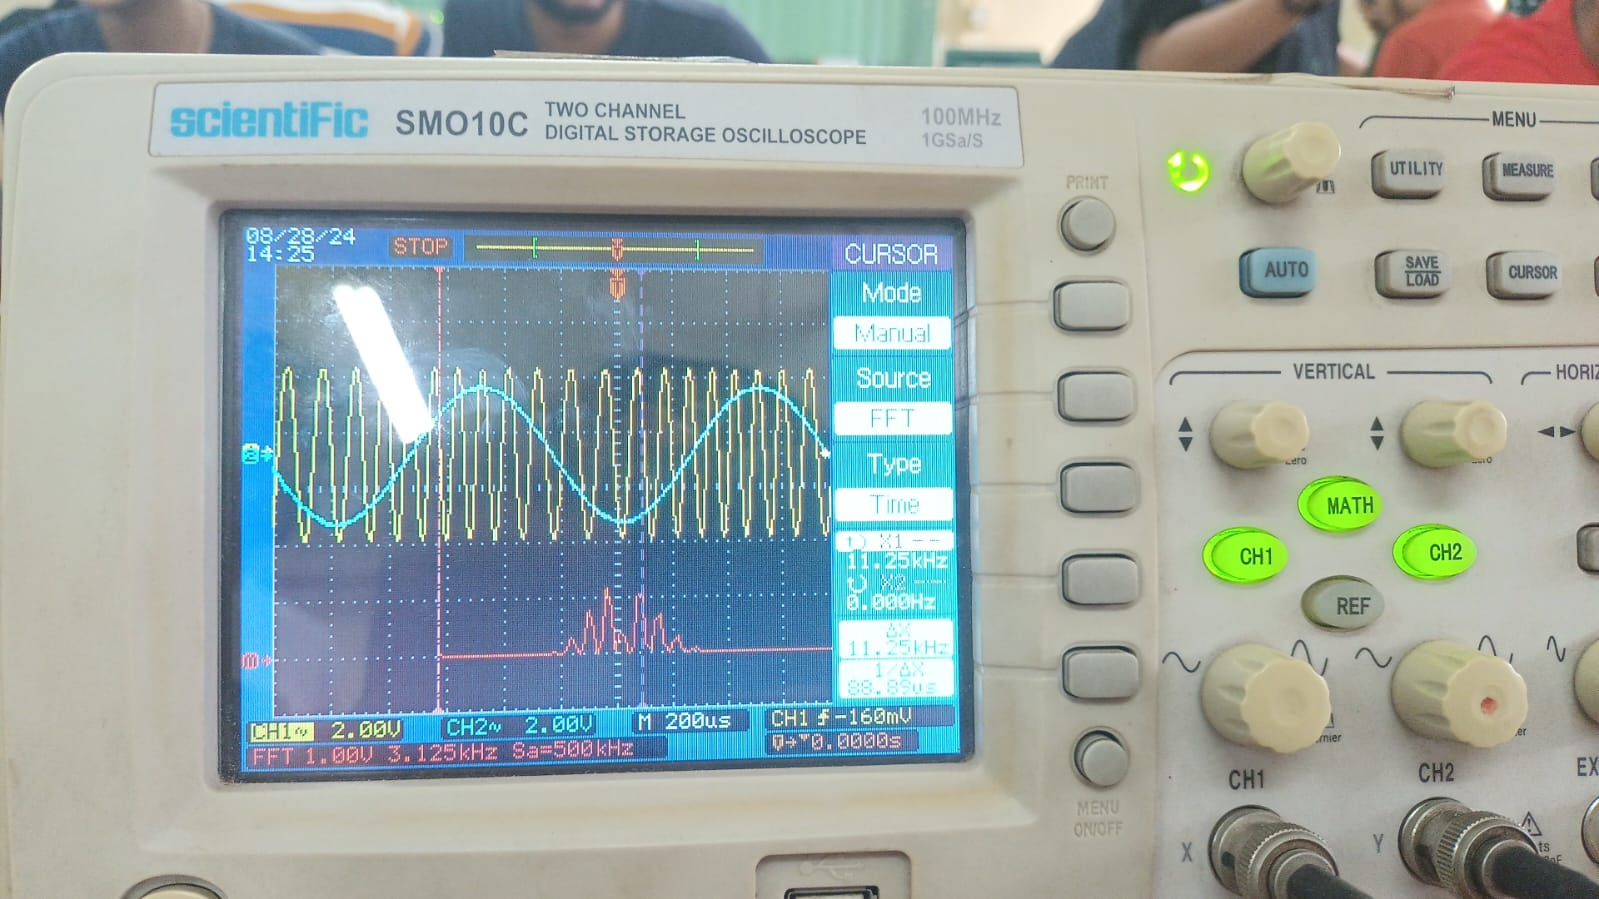
\includegraphics[width=\textwidth]{V_pp_m_3V.jpeg}
\caption{Final output and FFT with $V_{pp}=3V$ for the message}
\label{fig:V_pp_m_3V}
\end{figure}
\begin{equation}
    m=\frac{\Delta f}{f_m}=\frac{13.25-10.08}{1}=3.17
\end{equation}
\begin{figure}[!ht]
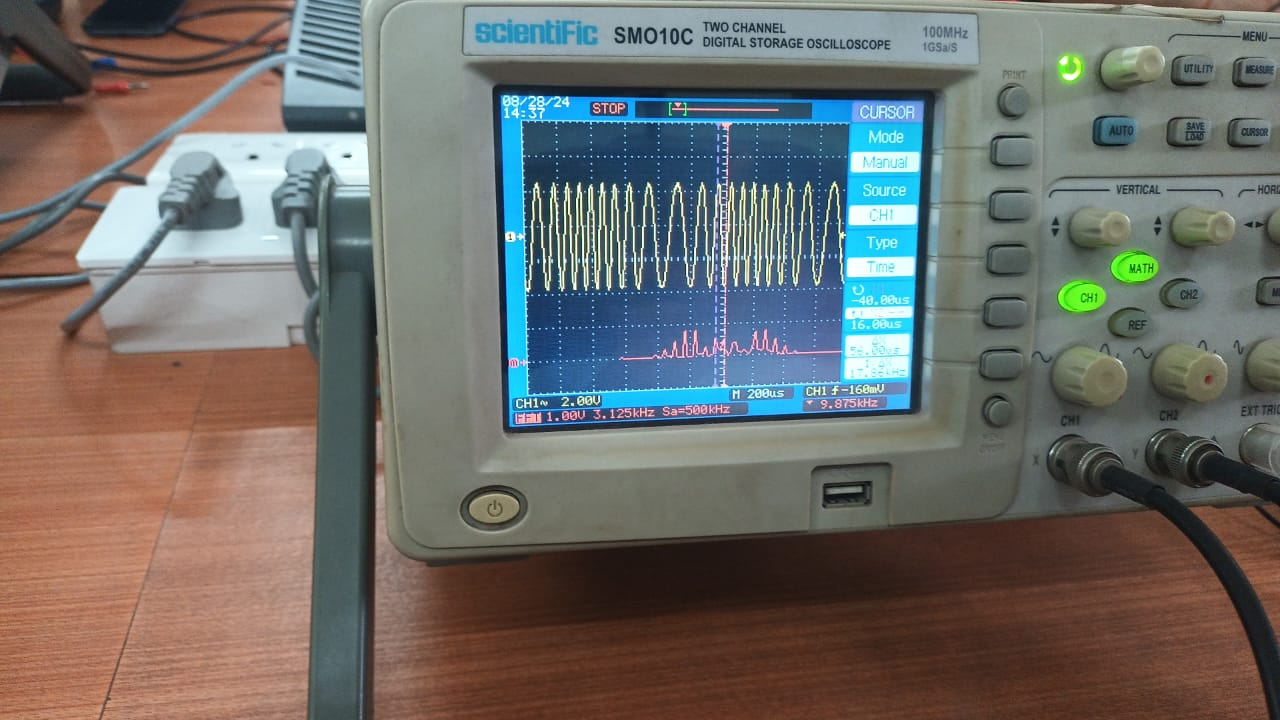
\includegraphics[width=\textwidth]{V_pp_m_7V.jpeg}
\caption{Final output and FFT with $V_{pp}=7V$ for the message}
\label{fig:V_pp_m_7V}
\end{figure}
\begin{equation}
    m=\frac{\Delta f}{f_m}=\frac{17.25-10.08}{1}=7.17
\end{equation}
\begin{figure}[!ht]
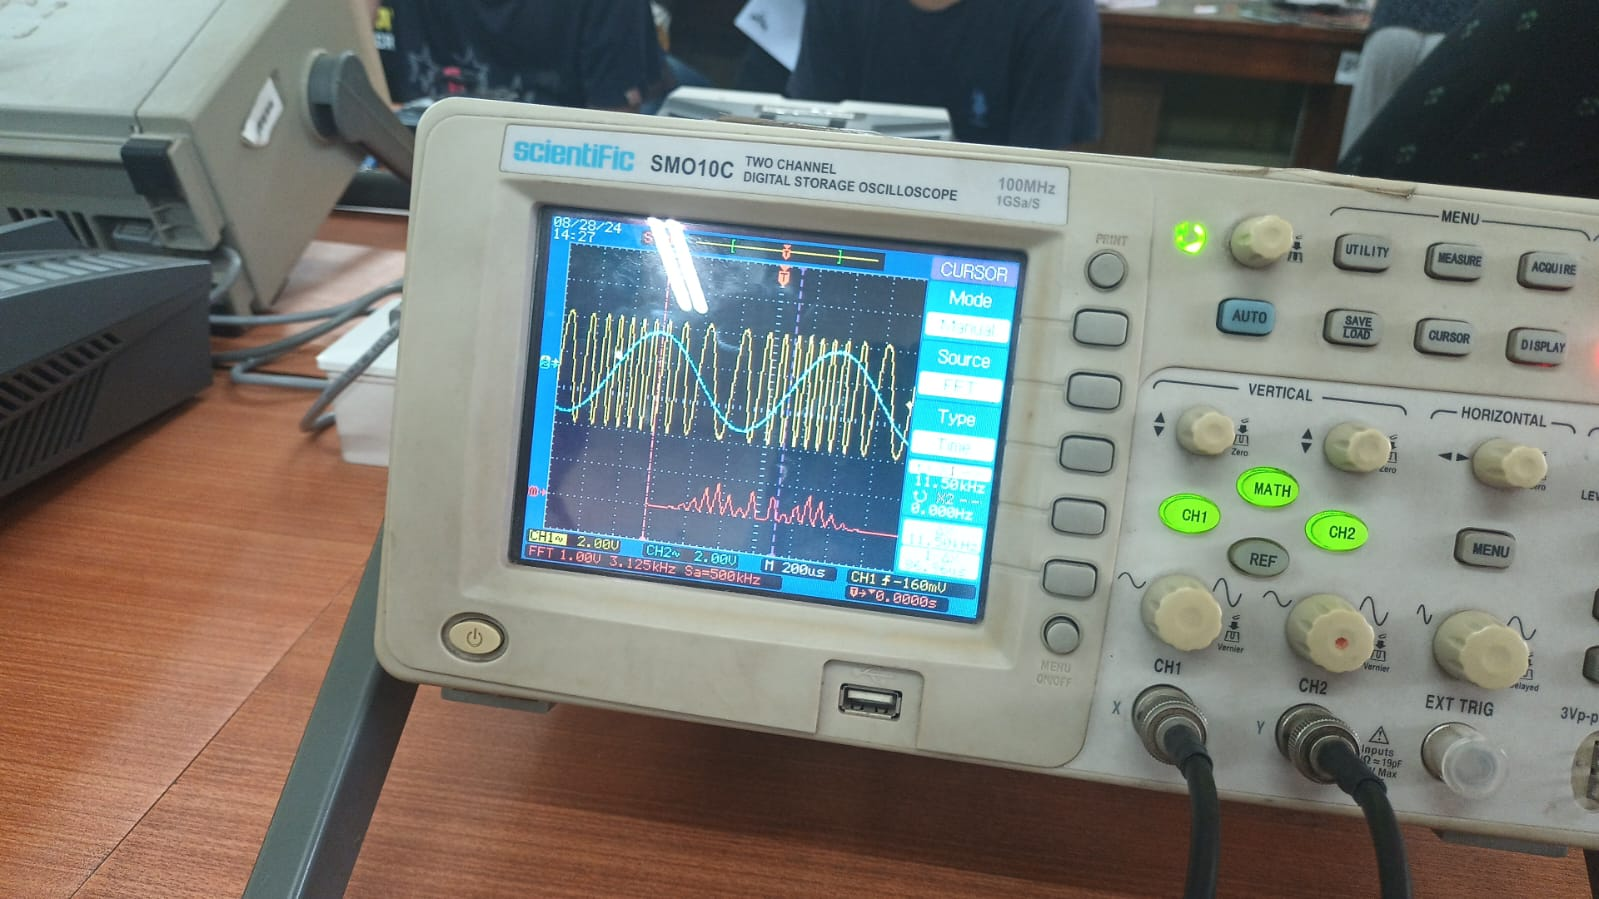
\includegraphics[width=\textwidth]{V_pp_m_8V.jpeg}
\caption{Final output and FFT with $V_{pp}=8V$ for the message}
\label{fig:V_pp_m_8V}
\end{figure}
\begin{equation}
    m=\frac{\Delta f}{f_m}=\frac{17.25-10.08}{1}=7.17
\end{equation}


\clearpage
\section{Discussion}
\subsection{Samyak Sheersh, 22EC30045}
\begin{enumerate}
  \item We saw that increasing the amplitude of the message gave a higher modulation index. This is because, as we can see from the expression for $f_i$, $\Delta f$ is larger when the amplitude of the message signal is larger. 
  \item We also saw that at larger amplitudes of the message, more harmonics were coming in the FFT. In the ideal case, we'll see that the harmonics will be stretching on all the way to $\infty$
  \item  Due to overmodulation, the peak at 10kHz gets suppressed
  \item Also, as we went above $10 V_{pp}$, the signals were no longer sinusoidal and thus weren't properly modulated.
  \item The XR 2206 is composed of 4 functional blocks: a voltage controlled oscillator, an analog multiplier and sine shaper, a unity gain buffer amplifier, and a set of current switches.
  \item The VCO produces an output frequency proportional to an input current, which a resistor sets from the timing terminals to the ground. We tune the potentiometer to adjust the output frequency, it provides the desired control voltage to the VCO for generating that frequency.
  \item By balancing the potentiometer, we generate the required carrier signal. It will set the appropriate control voltage to the VCO for generating that carrier frequency.
  \item And just like in the AM case, as the bias level approaches the $\frac{V_{dd}}{2}$ level, the carrier flips and thus, the phase inversion that we see in the output.
\end{enumerate}
\end{document}
%
